\documentclass[10pt]{IEEEtran}
\usepackage[spanish]{babel}
\usepackage[utf8]{inputenc}
\usepackage{graphicx}
\DeclareGraphicsExtensions{.bmp,.png,.pdf,.jpg}
\usepackage{amsmath}


\title {Caos y criptografía.}



\author{\IEEEauthorblockN{Marcos Daniel Calderón Calderón}\\
\IEEEauthorblockA{Maestría en Ciencias de la Computación\\
Centro de Investigación en Matemáticas (CIMAT)\\
Guanajuato , Gto.\\
marcos.calderon@cimat.mx}}


\begin{document}
\maketitle
\begin{abstract}
Resumen del artículo ''Caos y Criptografía.''
\end{abstract}

\section{Introduccion.}

El día de hoy, la encriptación caótica está casi exclusivamente considerada dentro de la comunidad de sistemas no lineales. Antes, los sitemas lineales mostraban inconvenientes. Hoy, la opinión negativa sobre las aplicaciones de la encriptación caótica ya no es tan fuerte. 


\section{Terminología.}
La criptografía convencional trabaja en criptosisitemas que manejan valores discretos en un tiempo discreto. Aquí se incluye la criptografía clásica. El punto crucial en criptografía caótica es que se utiliza información contínua y se usan sistemas de valores contínuos, los cuales pueden operar en tiempo discreto o contínuo. Para enfatizar la diferencia entre criptografía convencional, se utiliza el término continuous-value  cryptography  como un sinónimo de la criptografía caótica. 

 
\section{Historia de la Criptografía.}
Ha habido muchos métodos desde tiempos lejanos: el cifrado de César, el cifrado de Vigénere, etc. También, han surgido nuevos algoritmos de encriptación: DES, RSA. El trabajo de Shannon ha sido muy importante para su desarrollo. Tanto así, que la criptografía es una ciencia moderna.

A pesar de la relevancia de los sistemas discretos, ha habido intentos de aplicar métodos criptográficos a información contínua. Sistemas caóticos autónomos fueron usados para generar números pseudoaleatorios en implementaciones discretas.

Actualmente, los sistemas caóticos con señales contínuas se usan para transmitir información. Varios esquemas han sido desarrollados, lo cual permite transformar la información de las señales en una onda caótica cuando pasa por un codificador, y se puede extraer la información de la señal en el lado del decodificador. Los esquemas caóticos más importantes que se han desarrollado son los siguientes:

\begin{itemize}
\item \textbf{Máscara caótica.} La codificación consiste en un sistema caótico cuya señal de salida es agregada a la señal que representa la información, el resultado obtenido es transmitido en el canal de comunicación. El decodificador usa la señal que se ha transmitido sobre el canal. El decodificador usa la señal que se ha transmitido para sincronizarla con un sistema caótico equivalente al del decodificador. La señal caótica reconstruída es entonces restada de la señal de transmisión y esto nos da al final la señal original. Para garantizar sincronización, entonces, en el lado donde se resive la señal, ésta debe ser suficientemente pequeña con respecto a la señal caótica. 

\item \textbf{Chaos shift Keying.} La codificación consiste en dos o más sistemas caóticos autónomos con diferentes parámetros. De acuerdo a la información discreta (señal) uno de los sistemas caóticos es elegido y será transmitido sobre el canal. En el decodificador, el mismo número de sistemas caóticos se sincronizarán con los de su contraparte. Los parámetros son ajustados de tal manera que un par se sincroniza a la vez.
\item Modulación caótica o sistema inverso. EL codificador es un sistema caótico no autónomo cuyo estado es influenciado por la señal de la información. El decodificador sincroniza con el codificador por la reconstrucción de su estado usando la señal de transmisión.
\end{itemize}


\textbf{Bases de la criptografía.}\\
\begin{itemize}
\item \textbf{Criptosistema simétrico de llave pública.} Estos sistemas están formados por el texto plano P, el espacio de cifrado C, el conjunto de llaves K, el conjunto de transformadas para el cifrado y descifrado.

\item \textbf{Criptosistema de estructura pública.} Un oponenete conoce la estructura del sistema de encriptación y la probabilidad a priori de la llave k que está siento utilizada. Para cualquier transmisión encriptada, el emisor y el receptor conocen a priori la llave utilizada y debe ser mantenida en secreto para cualquier otra persona.
\end{itemize}


\textbf{Seguridad.}\\
La medida de seguridad de un criptosistema de llave pública se basa en la capacidad de resistir los ataques de un oponente que tiene conocimiento sobre el texto plano. La seguridad de un criptosistema es evaluada por el promedio de ataques que se utilizan para romper el sistema. EL propósito de un ataque es conocer la llave utilizada que permite al enemigo encontrar la función de desencriptaje y así descifrar textos cifrados siempre que el texto esté encriptado con la misma llave.


\section{Sistemas caóticos en criptografía.}
Los sistemas caóticos caóticos para criptografía se pueden clasificar en los siguientes:
\begin{enumerate}
\item Máscara caótica.

Una máscara caótica muy común es conocido como ''mapa logístico'', que es una función matemática de recurrencia que representa a un modelo demográfico que trata de explicar la dinámica de una población donde se supone que el crecimiento de la población es cada vez más lento a medida que se acerca una cantidad de individuos considerada como límite.

Se comprobó que al cambiar los valores del único parámetro del modelo, éste presentaba soluciones muy distintas y a veces muy complejas. Por tal motivo, se puede decir que este modelo tiene un comportamiento caótico.

La siguiente gráfica nos muestra los valores que se generan al aplicar la siguiente ecuación de recurrencia:


\begin{equation*}
\begin{aligned}
x_{n+1}= x_{n}+rx_{n}(1-x_{n})
\end{aligned}
\end{equation*}

En la expresión anterior,  $x_{n}$ es un número entre cero y uno, cuando se presentó el modelo anterior, este valor represenmtaba una fracción de individuos en un territorio, respecto de un valor $n$ que se supone que sería el máximo número de individuos que pueden convivir. También, $r$ es un número positivo que representa la relación o tasa combinada entre la reproducción y la mordandad. En esta ecuación lineal, se describen dos efectos:

\begin{itemize}
\item EL crecimiento de la población es exponencial.
\item La mortalidad adicional aumenta cuando crece la población, debido a la competencia de los individuos entre sí para asegurarse sus alimentos.
\end{itemize}
\begin{figure}[h]
\centering
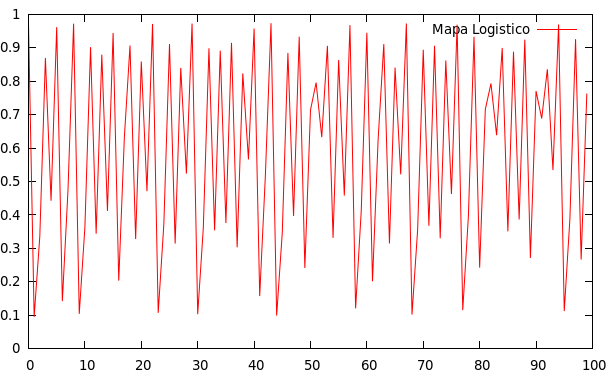
\includegraphics[width=8cm]{ss.png}
\caption{Valores obtenidos con un esquema caótico.}
\label{valores}
\end{figure}

\item Desplazamiento de llave caótica.
\item Sistemas inversos o modulación caótica.
\end{enumerate}

\section{Fundamentos de Criptología.}
\subsection*{Criptosistemas simétricos de canal público.}
Un criptosistema simétrico de canal público está formado por los siguientes componentes:
\begin{enumerate}
\item El conjunto de símbolos que conforman el texto plano $\rho.$
\item El conjunto de símbolos que conforman el texto cifrado $\zeta.$
\item El conjunto de llaves $k.$
\item Una función de encriptación $E$.
\item Una función de decriptación $D$.
\end{enumerate}

Los sistemas de encriptación pueden ser clasificados de acuerdo a las política manejadas sobre el manejo del sistema: si es conocida su forma de operación, la principal clasificación es la siguiente:

\begin{enumerate}
\item Sistemas de canal público. Un oponente puede acceder al canal de transmisión y puede conocer un fragmento del texto cifrado. 
\item Sistemas de estructura pública. Un oponente conoce la estructura del sistema de encriptación y  conoce una probabilidad a priori de acertar a la llave utilizada. En estos sistemas sólo se necesita que la llave utilizada sea secreta. 
\end{enumerate}

Actualmente, se utilizan muchos sistemas donde la llave $k$ determina la función de encriptación y también la función de decriptación. Antes de utlizar cualquier sistema criptográfico, el emisor y el receptor deben de conocer la llave que se va a utilizar, y sólo ellos la pueden conocer, para cualquier otra entidad la llave permanecerá secreta. Estos sistemas son conocidos como criptosistemas de llave secreta.


\subsection*{Ataques.}

Los ataques en estos sistemas se pueden clasificar en dos tipos:

\begin{itemize}
\item Cuando el intruso conoce una parte del texto cifrado.
\item CUando el intruso conoce el texto cifrado y el texto plano, con estos conocimientos, puede conocer la llave que se ha utilizado en este sistema.
\end{itemize}


\subsection*{Seguridad.}

La seguridad de un sistema de encriptación se mide con la capacidad que éste muestra para resistir los ataques de un enemigo. La seguridad de un criptosistema es evaluada por el promedio de ataques que se tienen que aplicar en un sistema para romperlo. El principal propósito de un ataque es determinar la llave utilizada, de esta manera, el intruso puede encontrar la función de encriptación  y así descifrar todos los textos cifrados que hayan utilizado este esquema.


\section{Esquemas de sincronización.}

\subsection*{Cifrado en bloques.}
Uu cifrado de bloque es una transformación estática de la siguiente forma: $F_{B}= W_{P} \longrightarrow W_{C} $, este tipo de cifrado opera en el texto plano segmentado $p= {p_{0}, p_{1}, p_{2},...}$ en donde cada ploque del texto plano $p_{i} \in W_{P}$ es encriptado independientemente de todos los demás bloques.


\begin{equation*}
\begin{aligned}
 F_{B}: \left\lbrace p_{0}, p_{1},p_{2},... \right\rbrace  \longrightarrow \left\lbrace F_{B}(p_{0}), F_{B}(p_{1}),F_{B}(p_{2}),...\right\rbrace 
\end{aligned}
\end{equation*}

En la expresión anterior, $W_{P}$ y $W_{C}$ denotan el dominio del texto plano  y los bloques del texto cifrado, cada uno de estos conjuntos tiene longitudaes $L_{P}$ y  $L_{C}$ respectivamente. De esta manera, cada bloque de texto plano $p_{i}$ consiste de $L_{P}$ símbolos $s_{i,j}  \in W_{S}$
\begin{equation*}
\begin{aligned}
p_{i}=\left\lbrace   s_{i,0},s_{i,1},s_{i,2},...,s_{i, L_{p-1}}   \right\rbrace \in W_{p}= W_{S}^{L_{P}}
\end{aligned}
\end{equation*}


\subsection*{Cifrado en flujos.}
En muchas situaciones, una sola aplicacion de transforamciones estáticas no es suficient para cumplir con los requerimientos de encirptación. Esto ocurre especialmente cuando el tamaño del bloque es pequeño, por ejemplo si $L=1$, con el fin de robustecer tales tipos de cifrado, se han configurado sistemas dinámicos que cuentan con memoria $T$, y una función de combinación  $\phi(',')$ de tal manera que el  bloque del texto cifrado $c_{n}$, depende de un estado interno $z_{n}$ y posiblemente de todos los bloques cifradaos que han ocurrido hasta ahora. Las estructuras más importantes hasta ahora son la CFB y la OFB. Estos modos de operación también pueden ser considerados para valores continuos.





\section{Anexos.}
A continuación, se muestra un código de un ejemplo sencillo para el cifrado de Vigenére:
\begin{verbatim}
int main(int argc, char** argv) {
    
ifstream textoPlano( "alicia2.txt");
if (!textoPlano)
{
cerr<<"No se pudo abrir el archivo."<<endl;
exit( 1 );
} 


ofstream archivoSalida("enctriptado.txt");
if (!archivoSalida)
{
cerr<<"No se pudo abrir el archivo."<<endl;
exit( 1 );
} 


char c;

// Por el momento declaramos una
// llave en mayusculas.
unsigned char llave[]={'L','O','U','P'};

//Formamos la tabla de thritemius.
unsigned char **tablat=new unsigned char*[26];
for(int i =0; i<26; i++){
    tablat[i]= new unsigned char[26];
}
unsigned char valor;
for(int i =0; i<26; i++){
    for(int j =0; j<26; j++){
        valor=(65+i)+j;
        if(valor>90){
            valor-=26;
        }
        tablat[i][j]=valor;
    }
}

int posicion=0;
int posicionLlave=0;
unsigned char caracter1;
while((c=textoPlano.get())!=EOF){ 

    //Si el caracter de entrada
    // es una mayuscula...
        if((c>='A') &&( c<='Z')){
           //Obtenemos el caracter
           //pero ya cifrado.
            if(posicion>25){
                posicion-=26;
            }
            
            if(posicionLlave>3){
              posicionLlave-=4;
            }
                
           caracter1=
           tablat[c-65][llave[posicionLlave]-65];  
           archivoSalida<<caracter1;
           posicion++;
           posicionLlave++;
          }
        else{
          archivoSalida<<c;
        }
    
  
      }
    
    //Cerramos los archivos.
    archivoSalida.close();
    textoPlano.close();
   return 0;
 }
\end{verbatim}

\end{document}



